\documentclass[]{article}
\usepackage{lmodern}
\usepackage{amssymb,amsmath}
\usepackage{ifxetex,ifluatex}
\usepackage{fixltx2e} % provides \textsubscript
\ifnum 0\ifxetex 1\fi\ifluatex 1\fi=0 % if pdftex
  \usepackage[T1]{fontenc}
  \usepackage[utf8]{inputenc}
\else % if luatex or xelatex
  \ifxetex
    \usepackage{mathspec}
    \usepackage{xltxtra,xunicode}
  \else
    \usepackage{fontspec}
  \fi
  \defaultfontfeatures{Mapping=tex-text,Scale=MatchLowercase}
  \newcommand{\euro}{€}
\fi
% use upquote if available, for straight quotes in verbatim environments
\IfFileExists{upquote.sty}{\usepackage{upquote}}{}
% use microtype if available
\IfFileExists{microtype.sty}{%
\usepackage{microtype}
\UseMicrotypeSet[protrusion]{basicmath} % disable protrusion for tt fonts
}{}
\usepackage[margin=1in]{geometry}
\usepackage{longtable,booktabs}
\usepackage{graphicx}
\makeatletter
\def\maxwidth{\ifdim\Gin@nat@width>\linewidth\linewidth\else\Gin@nat@width\fi}
\def\maxheight{\ifdim\Gin@nat@height>\textheight\textheight\else\Gin@nat@height\fi}
\makeatother
% Scale images if necessary, so that they will not overflow the page
% margins by default, and it is still possible to overwrite the defaults
% using explicit options in \includegraphics[width, height, ...]{}
\setkeys{Gin}{width=\maxwidth,height=\maxheight,keepaspectratio}
\ifxetex
  \usepackage[setpagesize=false, % page size defined by xetex
              unicode=false, % unicode breaks when used with xetex
              xetex]{hyperref}
\else
  \usepackage[unicode=true]{hyperref}
\fi
\hypersetup{breaklinks=true,
            bookmarks=true,
            pdfauthor={Petr Keil, pkeil@seznam.cz},
            pdftitle={Template for writing scientific papers in R markdown},
            colorlinks=true,
            citecolor=blue,
            urlcolor=blue,
            linkcolor=magenta,
            pdfborder={0 0 0}}
\urlstyle{same}  % don't use monospace font for urls
\setlength{\parindent}{0pt}
\setlength{\parskip}{6pt plus 2pt minus 1pt}
\setlength{\emergencystretch}{3em}  % prevent overfull lines
\setcounter{secnumdepth}{5}

%%% Use protect on footnotes to avoid problems with footnotes in titles
\let\rmarkdownfootnote\footnote%
\def\footnote{\protect\rmarkdownfootnote}

%%% Change title format to be more compact
\usepackage{titling}
\setlength{\droptitle}{-2em}
  \title{Template for writing scientific papers in R markdown}
  \pretitle{\vspace{\droptitle}\centering\huge}
  \posttitle{\par}
  \author{Petr Keil, \href{mailto:pkeil@seznam.cz}{\nolinkurl{pkeil@seznam.cz}}}
  \preauthor{\centering\large\emph}
  \postauthor{\par}
  \predate{\centering\large\emph}
  \postdate{\par}
  \date{11/1/2015}




\begin{document}

\maketitle


\section{Abstract}\label{abstract}

\emph{Lorem ipsum dolor sit amet, est ad doctus eligendi scriptorem. Mel
erat falli ut. Feugiat legendos adipisci vix at, usu at laoreet
argumentum suscipiantur. An eos adhuc aliquip scriptorem, te adhuc dolor
liberavisse sea. Ponderum vivendum te nec, id agam brute disputando
mei.}

\section{Introduction}\label{introduction}

Lorem ipsum dolor sit amet, est ad doctus eligendi scriptorem. Mel erat
falli ut. Feugiat legendos adipisci vix at, usu at laoreet argumentum
suscipiantur. An eos adhuc aliquip scriptorem, te adhuc dolor
liberavisse sea. Ponderum vivendum te nec, id agam brute disputando mei.

Putant numquam tacimates at eum. Aliquip torquatos ex vis, mei et quando
debitis appareat, impetus accumsan corrumpit in usu. Nam mucius facilis
singulis id, duo ei autem imperdiet instructior. Cu ceteros alienum mel,
id vix putant impedit, ex idque eruditi forensibus eum. Posse dicunt id
usu. Ei iracundia constituto sed, duo ne exerci ignota, an eum unum
conceptam.

Has audire salutandi no, ut eam dicat libris dicunt. Pri hendrerit
quaerendum adversarium ea, dicat atqui munere et sea. Illum insolens eos
ne, eu enim graece rationibus mea. At postea utamur mel, eius nonumes
percipitur at vis. Numquam similique in per, te quo saepe utroque
pericula.

Ea nonumy volumus usu, no mel inermis dissentias. Dico partiendo
vituperatoribus eum et. Mea accusam convenire te, usu populo qualisque
gloriatur ut. Eu eum oratio altera option, ad mea ignota scriptorem. Ne
suas latine vix, eos oblique sanctus pertinax cu.

\section{Methods}\label{methods}

Lorem ipsum dolor sit amet, est ad doctus eligendi scriptorem. Mel erat
falli ut. Feugiat legendos adipisci vix at, usu at laoreet argumentum
suscipiantur. An eos adhuc aliquip scriptorem, te adhuc dolor
liberavisse sea. Ponderum vivendum te nec, id agam brute disputando mei.

Putant numquam tacimates at eum. Aliquip torquatos ex vis, mei et quando
debitis appareat, impetus accumsan corrumpit in usu. Nam mucius facilis
singulis id, duo ei autem imperdiet instructior. Cu ceteros alienum mel,
id vix putant impedit, ex idque eruditi forensibus eum. Posse dicunt id
usu. Ei iracundia constituto sed, duo ne exerci ignota, an eum unum
conceptam.

\subsection{Equations}\label{equations}

The deterministic part of the model is defined by this \textbf{in-line
equation} as \(\mu_i = \beta_0 + \beta_1x\), and the stochastic part by
the \textbf{centered equation}:

\[ \frac{1}{\sqrt{2\pi}\sigma}e^{-(x-\mu_i)^2/(2\sigma^2)} \]

\subsection{Tables}\label{tables}

\begin{longtable}[c]{@{}lrrrr@{}}
\caption{This is a GLM summary table.}\tabularnewline
\toprule
& Estimate & Std. Error & t value &
Pr(\textgreater{}\textbar{}t\textbar{})\tabularnewline
\midrule
\endfirsthead
\toprule
& Estimate & Std. Error & t value &
Pr(\textgreater{}\textbar{}t\textbar{})\tabularnewline
\midrule
\endhead
(Intercept) & 0.03 & 0.1 & 0.31 & 0.76\tabularnewline
x & 2.27 & 0.1 & 23.23 & 0.00\tabularnewline
\bottomrule
\end{longtable}

\subsection{Plots}\label{plots}

\begin{figure}[htbp]
\centering
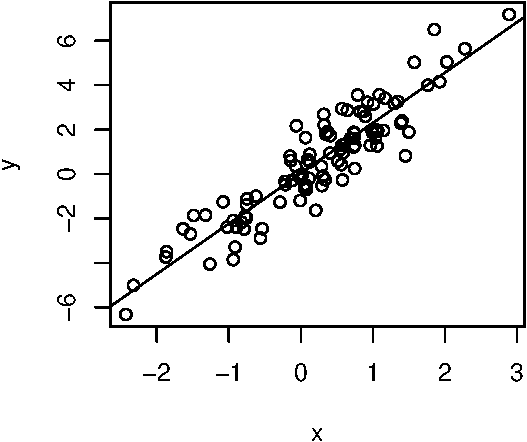
\includegraphics{manuscript_template_files/figure-latex/carDataPlot-1.pdf}
\caption{Relationship between x and y. The solid line is least-squares
linear regression.}
\end{figure}

\subsection{Citations}\label{citations}

The relationship was first described by Halpern et al. (2006). However,
there are also opinions that the relationship is spurious (Keil \emph{et
al.} 2012). We used R for our calculations (R Core Team 2015), and we
used package \texttt{knitcitations} (Boettiger 2015) to make the
bibliography.

\section{Results and discussion}\label{results-and-discussion}

Lorem ipsum dolor sit amet, est ad doctus eligendi scriptorem. Mel erat
falli ut. Feugiat legendos adipisci vix at, usu at laoreet argumentum
suscipiantur. An eos adhuc aliquip scriptorem, te adhuc dolor
liberavisse sea. Ponderum vivendum te nec, id agam brute disputando mei.

Putant numquam tacimates at eum. Aliquip torquatos ex vis, mei et quando
debitis appareat, impetus accumsan corrumpit in usu. Nam mucius facilis
singulis id, duo ei autem imperdiet instructior. Cu ceteros alienum mel,
id vix putant impedit, ex idque eruditi forensibus eum. Posse dicunt id
usu. Ei iracundia constituto sed, duo ne exerci ignota, an eum unum
conceptam.

Has audire salutandi no, ut eam dicat libris dicunt. Pri hendrerit
quaerendum adversarium ea, dicat atqui munere et sea. Illum insolens eos
ne, eu enim graece rationibus mea. At postea utamur mel, eius nonumes
percipitur at vis. Numquam similique in per, te quo saepe utroque
pericula.

Ea nonumy volumus usu, no mel inermis dissentias. Dico partiendo
vituperatoribus eum et. Mea accusam convenire te, usu populo qualisque
gloriatur ut. Eu eum oratio altera option, ad mea ignota scriptorem. Ne
suas latine vix, eos oblique sanctus pertinax cu.

\section*{References}\label{references}
\addcontentsline{toc}{section}{References}

Boettiger, C. (2015). \emph{Knitcitations: Citations for knitr markdown
files}. Retrieved from \url{https://github.com/cboettig/knitcitations}

Halpern, B.S., Regan, H.M., Possingham, H.P. \& McCarthy, M.A. (2006).
Accounting for uncertainty in marine reserve design. \emph{Ecol
Letters}, \textbf{9}, 2--11. Retrieved from
\url{http://dx.doi.org/10.1111/j.1461-0248.2005.00827.x}

Keil, P., Belmaker, J., Wilson, A.M., Unitt, P. \& Jetz, W. (2012).
Downscaling of species distribution models: A hierarchical approach (R.
Freckleton, Ed.). \emph{Methods Ecol Evol}, \textbf{4}, 82--94.
Retrieved from \url{http://dx.doi.org/10.1111/j.2041-210x.2012.00264.x}

R Core Team. (2015). \emph{R: A language and environment for statistical
computing}. R Foundation for Statistical Computing, Vienna, Austria.
Retrieved from \url{http://www.R-project.org/}

\end{document}
